\documentclass[11pt,a4paper,modern]{MWExercises}
\usepackage[english,greek]{babel}
\usepackage[utf8]{inputenc}
\usepackage{fontspec}
 
\setmainfont{Minion Pro}
\newfontfamily{\century}{Century Gothic}
\usepackage{amsmath,svg,diffcoeff,fancyhdr,lipsum}
\let\myBbbk\Bbbk
\let\Bbbk\relax
\usepackage[amsbb,subscriptcorrection,zswash,mtpcal,mtphrb,mtpfrak]{mtpro2}
\usepackage{graphicx,multicol,multirow,enumitem,tabularx,mathimatika,gensymb,venndiagram,hhline,longtable,tkz-euclide,fontawesome5,eurosym,tcolorbox,tabularray,tikzpagenodes,relsize}
\definecolor{xrwma}{HTML}{0094a8}%0094a8
\colorlet{darkxrwma1}{xrwma!70!black}
\colorlet{darkxrwma2}{xrwma!35!black}
\usetikzlibrary{calc}
\usetikzlibrary{positioning}
\tcbuselibrary{skins,theorems,breakable}
\renewcommand{\textstigma}{\textsigma\texttau}
\renewcommand{\textdexiakeraia}{}

\fancypagestyle{firstpage}{% define a custom header
  \fancyhf{}
\renewcommand{\headrulewidth}{0pt}
  \fancyfoot[CO]{
\begin{tikzpicture}[overlay, remember picture]%
\fill[xrwma] ($(current page.south)+(-1.2,0)$) -- ($(current page.south)+(-0.7,0.5)$)
-- ($(current page.south)+(0.7,0.5)$)-- ($(current page.south)+(1.2,0)$)--cycle;
\node[anchor=south, text=white] at (current page.south) {\thepage};
\fill[xrwma] (current page.south west) rectangle ($(current page.south west)+(0.7,1.2)$);
\fill[xrwma] (current page.south east) rectangle ($(current page.south east)+(-0.7,1.2)$);
\node[color=white] at ($(current page.south west)+(0.35,0.85)$) {\faMobile*};
\node[color=white] at ($(current page.south west)+(0.35,0.35)$) {\faEnvelope[regular]};
\node[color=white] at ($(current page.south east)+(-0.35,0.85)$) {\faInstagram};
\node[color=white] at ($(current page.south east)+(-0.35,0.35)$) {\faFacebook};

\node[anchor=west] at ($(current page.south west)+(0.85,0.85)$) {26610 20144 - 693 232 7283};
\node[anchor=west] at ($(current page.south west)+(0.85,0.35)$) {{\eng{frontistirio.filomatheia@gmai.com}}};
\node[anchor=east] at ($(current page.south east)+(-0.85,0.85)$) {{\eng{front\_filomatheia}}};
\node[anchor=east] at ($(current page.south east)+(-0.85,0.35)$) {Φροντιστήριο Φιλομάθεια};
\end{tikzpicture}
}
}

\pagestyle{fancy}
\fancyhf{}
\fancyhead[R]{\century{{\footnotesize Παράγωγος Συνάρτηση}}}
  \fancyhead[L]{\century{{\footnotesize Μαθηματικά Γ' Λυκείου}}}
\fancyfoot[CO]{
\begin{tikzpicture}[overlay, remember picture]%
\fill[xrwma] ($(current page.south)+(-1.2,0)$) -- ($(current page.south)+(-0.7,0.5)$)
-- ($(current page.south)+(0.7,0.5)$)-- ($(current page.south)+(1.2,0)$)--cycle;
\node[anchor=south, text=white] at (current page.south) {\thepage};
\fill[xrwma] (current page.south west) rectangle ($(current page.south west)+(0.7,1.2)$);
\fill[xrwma] (current page.south east) rectangle ($(current page.south east)+(-0.7,1.2)$);
\node[color=white] at ($(current page.south west)+(0.35,0.85)$) {\faMobile*};
\node[color=white] at ($(current page.south west)+(0.35,0.35)$) {\faEnvelope[regular]};
\node[color=white] at ($(current page.south east)+(-0.35,0.85)$) {\faInstagram};
\node[color=white] at ($(current page.south east)+(-0.35,0.35)$) {\faFacebook};

\node[anchor=west] at ($(current page.south west)+(0.85,0.85)$) {26610 20144 - 693 232 7283};
\node[anchor=west] at ($(current page.south west)+(0.85,0.35)$) {{\eng{frontistirio.filomatheia@gmai.com}}};
\node[anchor=east] at ($(current page.south east)+(-0.85,0.85)$) {{\eng{front\_filomatheia}}};
\node[anchor=east] at ($(current page.south east)+(-0.85,0.35)$) {Φροντιστήριο Φιλομάθεια};
\end{tikzpicture}
}

\ekthetesdeiktes



\begin{document}
\thispagestyle{firstpage}
\begin{tikzpicture}[overlay,remember picture]
\tikzset{
	bigrect/.style = {rectangle, minimum width=3mm,minimum height=3mm, fill=xrwma, opacity=0.4},
	rect/.style = {rectangle, minimum width=2mm,minimum height=2mm, fill=xrwma, opacity=0.4},
	smallrect/.style = {scale=0.7,rectangle, minimum width=1mm,minimum height=1mm, fill=xrwma, opacity=0.4}
}
%-------- Logo - Layout ---------------
\fill[xrwma,rounded corners=2pt,yshift=11mm] (30:0.75) -- (0,0) -- (270:0.75) -- (330:0.75)--cycle;
\fill[xrwma!85!black,rounded corners=2pt,yshift=11mm] (30:0.75) -- (90:0.75) -- (150:0.75) -- (0,0)--cycle;
\fill[xrwma!70!black,rounded corners=2pt,yshift=11mm] (150:0.75) -- (210:0.75) -- (270:0.75) -- (0,0)--cycle;
\draw[line width=.5mm,white,yshift=11mm] (0,0) -- (270:0.75);
\draw[line width=.5mm,white,yshift=11mm] (0,0) -- (30:0.75);
\draw[line width=.5mm,white,yshift=11mm] (0,0) -- (150:0.75);
\node at ($(current page.north west)+(4.3,-1.3)$) {\century{{\fontsize{20}{24}\selectfont \textcolor{xrwma}{\textbf{Φιλομάθεια}}}}};
\node at ($(current page.north west)+(4.3,-0.8)$) {{\scriptsize\fontsize{0.8em}{0.98em} \century{ΦΡΟΝΤΙΣΤΗΡΙΟ ΜΕΣΗΣ ΕΚΠΑΙΔΕΥΣΗΣ}}};
\node at ($(current page.north west)+(4.3,-1.8)$) {{\footnotesize\fontsize{0.82em}{0.98em}\selectfont \textcolor{xrwma}{\faMapMarker*} Ιακώβου Πολυλά 24 - Πεζόδρομος}};
\fill[xrwma!35!black] ($(current page.north west)+(9.2,-2.5)$)--($(current page.north west)+(0,-2.5)$)--($(current page.north west)+(0,-2.8)$)--($(current page.north west)+(8.6,-2.8)$)--cycle;
\path[step=0.5,right color=xrwma,left color=white] ($(current page.north east)$) grid ($(current page.north east)+(-8.4,-2.7)$);
\path[step=0.1,opacity=1,right color=xrwma,left color=white,thin] ($(current page.north east)$) grid ($(current page.north east)+(-8.4,-2.7)$);
%------------ Title ------------------
\node[anchor=west] at($(current page.north west)+(1,-3.8)$) {\textcolor{xrwma}{\Large \century{Μαθηματικά Γ' Λυκείου}}};
\node[anchor=west] at($(current page.north west)+(1,-4.3)$) {\textcolor{darkxrwma2}{\large \century{Διαφορικός Λογισμός}}};

\node[anchor=east] at($(current page.north east)+(-1,-3.8)$){\century{Παράγωγος Συνάρτηση}};
\node[anchor=east] at($(current page.north east)+(-1,-4.3)$) {\century{{Φυλλάδιο Ασκήσεων}}};
\node at($(current page.north)+(0,-4.8)$) {\century{\textbf{Φυλλάδιο Ασκήσεων}}};

%---------- Squares ----------------
\node[bigrect] at (15.5,0.7){};
\node[bigrect] at (15,1){};
\node[bigrect] at (14.9,2.1){};
\node[bigrect] at (13.7,.8){};
\node[bigrect] at (14.1,1.7){};
\node[bigrect] at (14.1,1.15){};
\node[bigrect] at (14.5,1.3){};
\node[rect] at (12.6,1.5){};
\node[rect,scale=0.8] at (12.6,1.9){};
\node[rect] at (13.38,1.65){};
\node[rect] at (13.1,1.2){};
\node[rect,scale=0.8] at (12.1,1.7){};
\node[rect] at (15.2,1.5){};
\node[rect] at (16.9,1.63){};
\node[rect] at (16.4,0.7){};
\node[smallrect] at (13.7,1.4){};
\node[smallrect,scale=0.8] at (11.4,1.57){};
\node[smallrect] at (10.9,1.4){};
\node[smallrect] at (11.7,1.42){};
\node[smallrect,scale=0.7] at (11.4,1.2){};
\node[smallrect] at (12.9,0.8){};
\node[smallrect] at (12,1){};
\node[smallrect] at (12.3,1.2){};
\node[smallrect] at (12.6,1){};
\node[smallrect,scale=0.8] at (12.9,1.7){};
\node[smallrect] at (13.4,1){};
\node[smallrect] at (15,.4){};
%------------- Formulas ------------------------
\node at ($(current page.north east)+(-1.4,-0.7)$){\color{darkxrwma2}{$\displaystyle\int_{0}^{\infty}{\!\!\!f(x)\mathrm{d}x}$}};
\node at ($(current page.north east)+(-4.4,-.85)$){\color{darkxrwma2}{$\displaystyle\iiint_{D}{\nabla\cdot \mathbold{F}\mathrm{d}V}$}};
\node at ($(current page.north east)+(-4.1,-2.3)$){{\tiny \color{darkxrwma1}{$\displaystyle\diffp[n,m]{f(x,y)}{x,y}$}}};
\node at ($(current page.north east)+(-5.4,-1.8)$){{\scriptsize \color{xrwma}{$\displaystyle\lim_{x\to x_0}{f(x)}$}}};
\node at ($(current page.north east)+(-3.5,-1.5)$){{\small \color{darkxrwma2}{$\displaystyle\sum_{n=1}^{\infty}{\frac{1}{n^2}}=\frac{\pi^2}{6}$}}};
\node at ($(current page.north east)+(-1.5,-2.2)$){\color{darkxrwma2}{$\displaystyle\liminf_{n\to\infty}{a_n}=l$}};
\node at ($(current page.north east)+(-1.4,-1.5)$){\color{darkxrwma2}{$\displaystyle u_t=\kappa\nabla^2u$}};
\node at ($(current page.north east)+(-2,-1)$){{\footnotesize \color{xrwma}{$\displaystyle x^2y''+xy'+y=p(x)$}}};
\node at ($(current page.north east)+(-3,-.4)$){{\tiny \color{xrwma}{$\displaystyle F(k)=\int_{-\infty}^{\infty}{f(x)e^{-2\pi ikx}\mathrm{d}x}$}}};
%--------------- Right rule --------------------
\fill[xrwma] ($(current page.north east)+(-8.6,-2.5)$)--($(current page.north east)+(0,-2.5)$)--($(current page.north east)+(0,-2.8)$)--($(current page.north east)+(-9.2,-2.8)$)--cycle;
\end{tikzpicture}
\mbox{}\\\vspace{2.5cm}\\
Συνάρτηση ονομάζεται ο κανόνας (αντιστοίχηση) με τον οποίο \textbf{κάθε} στοιχείο ενός συνόλου $ A $ αντιστοιχεί σε \textbf{ένα μόνο} στοιχείο ενός συνόλου $ B $.\\Συμβολίζεται με οποιοδήποτε γράμμα του λατινικού ή και του ελληνικού αλφαβήτου $ f, g, h, t, s, \sigma\ldots $ και γράφουμε : \[ f:A\rightarrow B \]
Είναι η σχέση που συνδέει δύο μεταβλητές $ x,y $ όπου κάθε τιμή της πρώτης $ (x\in A) $, στο πρώτο σύνολο, αντιστοιχεί σε μόνο μια τιμή της δεύτερης $ (y\in B) $, στο δεύτερο σύνολο.\vspace{-3mm}
\begin{center}
\begin{figure}[h]
\centering
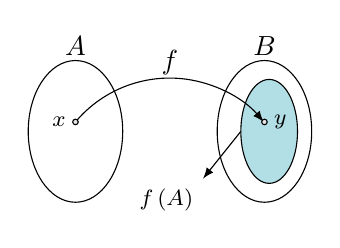
\begin{tikzpicture}[scale=.6]
\draw(0,0) ellipse (1cm and 1.5cm);
\draw(4,0) ellipse (1cm and 1.5cm);
\draw[fill=xrwma!30] (4.1,0) ellipse (.6cm and 1.1cm);
\draw[-latex] (0,.2) arc (140:40:2.6);
\tkzDefPoint(0,.2){A}
\tkzDefPoint(4,.2){B}
\tkzDrawPoints(A,B)
\tkzLabelPoint[left](A){{\footnotesize $ x $}}
\tkzLabelPoint[right](B){{\footnotesize $ y $}}
\tkzText(0,1.8){$ A $}
\tkzText(4,1.8){$ B $}
\tkzText(2,1.45){$ f $}
\draw[-latex] (3.5,0) -- (2.7,-1) node[anchor=north east] {\footnotesize $ f\left( A \right)  $};
\end{tikzpicture}
\end{figure}
\end{center}
\vspace{-1.1cm}
\begin{itemize}[itemsep=0mm]
\item Η μεταβλητή $ x $ του συνόλου $ A $ ονομάζεται \textbf{ανεξάρτητη} ενώ η $ y $ \textbf{εξαρτημένη}.
\item Η τιμή της $ y $ ονομάζεται \textbf{τιμή} της $ f $ στο $ x $ και συμβολίζεται $ y=f(x) $.
\item Ο κανόνας της συνάρτησης, με τον οποίο γίνεται η αντιστοίχηση από το $ x $  στο $ f(x) $, εκφράζεται συμβολικά με τη βοήθεια του $ x $ και ονομάζεται \textbf{τύπος της συνάρτησης}.
\item Το σύνολο $ A $ λέγεται \textbf{πεδίο ορισμού} της συνάρτησης $ f $ και συμβολίζεται $ D_f $. Είναι το σύνολο των δυνατών τιμών την ανεξάρτητης μεταβλητής της συνάρτησης.
\item Το σύνολο με στοιχεία όλες τις δυνατές τιμές $ f(x) $ της εξαρτημένης μεταβλητής για κάθε $ x\in D_f $ λέγεται \textbf{σύνολο τιμών} της $ f $, συμβολίζεται $ f\left(D_f\right) $ και ισχύει $ f\left(D_f\right)\subseteq B $.
\item Μια συνάρτηση συμβολίζεται επίσης με τους εξής τρόπους : \[ x\overset{f}{\mapsto}f(x)\;\;,\;\;D_f\overset{f}{\rightarrow}f\left(D_f\right) \]
\item Για το συμβολισμό της ανεξάρτητης μεταβλητής ή της συνάρτησης μπορούμε να χρησιμοποιήσουμε οποιοδήποτε συμβολισμό στη θέση της μεταβλητής $ x $ ή του ονόματος $ f $ της συνάρτησης αντίστοιχα. \[ f(x)\;\;,\;\;g(t)\;\;,\;\;h(s)\ldots \]
\vspace{-3mm}
\item Για να ορίσουμε μια συνάρτηση θα πρέπει να γνωρίζουμε
\vspace{-3mm}
\begin{enumerate}[itemsep=0mm]
\begin{multicols}{2}
\item To πεδίο ορισμού $ D_f $.
\item Το σύνολο $ B $.
\end{multicols}
\vspace{-3mm}
\item Τον τύπο $ f(x) $ της συνάρτησης, για κάθε $ x\in D_f $.
\end{enumerate}
\item Εαν τα σύνολα $ D_f,B $ είναι υποσύνολα του συνόλου των πραγματικών αριθμών τότε μιλάμε για \textbf{πραγματική συνάρτηση πραγματικής μεταβλητής}.
\item Οι συναρτήσεις των οποίων ο τύπος δίνεται από δύο ή περισσότερες αλγεβρικές παραστάσεις ονομάζονται συναρτήσεις \textbf{πολλαπλού τύπου}.
\[ f(x)=\ccases{f_1(x) & \textrm{αν }x\in D_{f_1}\subseteq D_f\\
f_2(x) & \textrm{αν }x\in D_{f_2}\subseteq D_f\\
\;\;\;\;\vdots & \qquad\vdots\\
f_\nu(x) & \textrm{αν }x\in D_{f_\nu}\subseteq D_f} \]
όπου $ D_{f_1},D_{f_2},\ldots,D_{f_\nu} $ είναι υποσύνολα του πεδίου ορισμού ολόκληρης της συνάρτησης $ f $ με $ D_{f_1}\cup D_{f_2}\cup \ldots\cup D_{f_\nu}=D_f $ και $  D_{f_1}\cap D_{f_2}\cap \ldots\cap D_{f_\nu}=\varnothing $.
\end{itemize}
Στον πίνακα βλέπουμε τα βασικά είδη συναρτήσεων τον τύπο τους και το πεδίο ορισμού τους.
\begin{center}
\begin{mytblr}{row{1}={font=\bfseries\century}}
{Είδος} & {Τύπος} & {Πεδίο Ορισμού} \\ 
 \textbf{Πολυωνυμική} & $ f(x)=a_\nu x^\nu+\ldots+a_1x+a_0 $ & $ D_f=\mathbb{R} $ \\
 \textbf{Ρητή} & $ f(x)=\dfrac{P(x)}{Q(x)} $ & $ D_f=\left\lbrace\left.  x\in\mathbb{R}\right| Q(x)\neq0\right\rbrace $  \\
 \textbf{Άρρητη} & $ f(x)=\sqrt{A(x)} $ & $ D_f=\left\lbrace\left. x\in\mathbb{R}\right| A(x)\geq0\right\rbrace $ \\
\SetCell[r=3,c=1]{c,m}\textbf{Τριγωνομετρική} & $ f(x)=\hm{x}\;\;,\;\;\syn{x} $ & $ D_f=\mathbb{R} $ \\ 
  & $ f(x)=\ef{x} $ & $ D_f=\left\lbrace\left.x\in\mathbb{R}\right| x\neq\kappa\pi+\frac{\pi}{2}\;,\;\kappa\in\mathbb{Z}\right\rbrace $ \\ 
  & $ f(x)=\syf{x} $ & $ D_f=\left\lbrace\left.x\in\mathbb{R}\right| x\neq\kappa\pi\;,\;\kappa\in\mathbb{Z}\right\rbrace $ \\ 
\textbf{Εκθετική} & $ f(x)=a^x\;\;,\;\;0<a\neq1 $ & $ D_f=\mathbb{R} $ \\ 
 \textbf{Λογαριθμική} & $ f(x)=\log{x}\;\;,\;\;\ln{x} $ & $ D_f=(0,+\infty) $ 
\end{mytblr}
\end{center}
\vspace{.8cm}
Επιπλέον, ειδικές περιπτώσεις πολυωνυμικών συναρτήσεων αποτελούν οι παρακάτω συναρτήσεις
\begin{center}
\begin{minipage}{2.5cm}
\textbf{Ταυτοτική}\\$ f(x)=x $
\end{minipage}\qquad
\begin{minipage}{2.5cm}
\textbf{Σταθερή}\\$ f(x)=c $
\end{minipage}\qquad
\begin{minipage}{2.5cm}
\textbf{Μηδενική}\\$ f(x)=0 $
\end{minipage}
\end{center}
\end{document}
